\documentclass[10pt]{article}
\usepackage[utf8]{inputenc}
%\usepackage[autostyle]{csquotes}
\usepackage[T1]{fontenc}
\usepackage{lmodern, alltt, color, geometry, multicol, eurosym, fancyhdr}
\usepackage{graphicx}
\usepackage[hyperindex=true, colorlinks=true, urlcolor=black, linkcolor=black, breaklinks=true]{hyperref}
\renewcommand*{\familydefault}{\sfdefault}
\pagestyle{empty}
\geometry{hmargin=1cm, vmargin=2cm}
\headsep 10pt
\setcounter{secnumdepth}{0}
\addtolength{\parskip}{6pt}
\renewcommand{\ttdefault}{pcr}
\setlength{\parindent}{0cm}
\pagestyle{fancy}
\fancyhead{}
\lfoot{}
\cfoot{\thepage{}}
\rfoot{}
\makeatletter
\makeatother

\title{On FOSS as a capitalism-like structure}
%\subtitle{Or, Time is Money}
\author{Cassian (@cassolotl)}
\date{June 8th, 2018}

\begin{document}

\maketitle

\begin{center}
\noindent\rule{8cm}{0.4pt}
\end{center}

\begin{multicols}{2}
Free and Open Source Software (FOSS) positions itself as being apart from capitalism. Software is written by people passionate about making their useful things freely available to all. Sometimes they’re paid but often they aren’t.

When they’re not, and when it’s a personal project that others may or may not contribute to, if someone using the software asks for a particular feature and the developer isn’t into the idea of adding it, the standard response is “you’re free to fork it and code whatever you want.” After all, that’s what FOSS is about.

If two people are equal in terms of coding ability and available time, that is a fair dynamic.

When someone is unable to code their options are:\footnote{It’s worth noting that there are disabilities that inherently and directly make (1) impossible and (3) very difficult, and anyone in a marginalised group is less likely to be able to do (2).}

\begin{enumerate}
\item Learn to code;
\item Pay someone else to code;
\item Find someone else who is willing and able to code for you for free.
\end{enumerate}

To put it another way:

\begin{center}
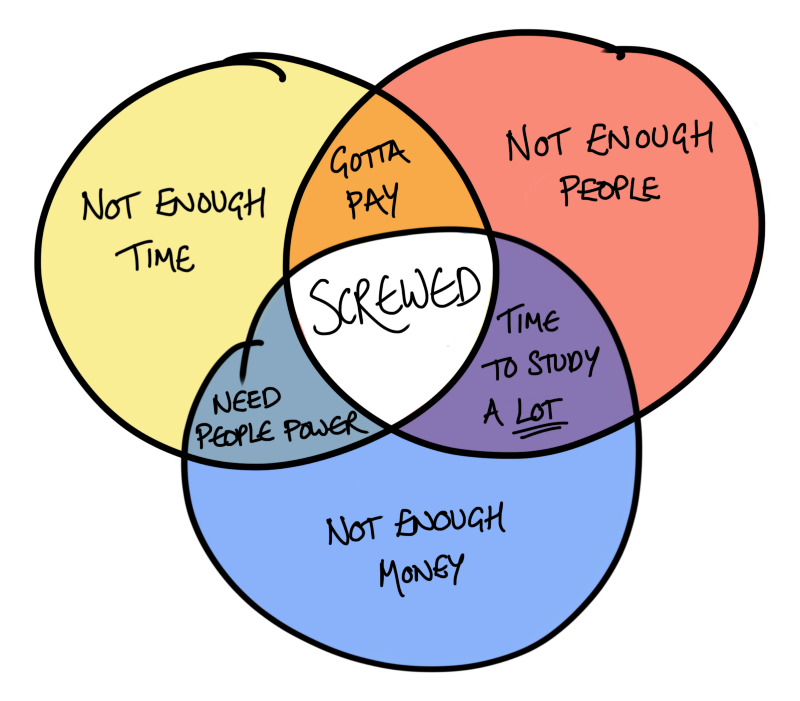
\includegraphics[width=0.33\textwidth]{foss-as-non-dev}\\
\emph{FOSS as a non-coder}
\end{center}

Time is money. If you have time you can use it to learn how to code, or to find skilled people and persuade them that it’s a good idea to work for you for free. If you lack time, you can often get around it by throwing money at it and buying someone else’s time. If you have enough people, everyone puts in less time each and things get done faster even though it’s still free.

Back to the project. If as a user you object to something about a particular FOSS program or the way a project is run, you will probably be told that you have the option of forking the project or choosing another fork or project that better suits your needs. This is considered a good thing, and forking projects is encouraged. But when you have no power it sucks.

Does this sound familiar?

“If you don’t like a company or product you can give your money or attention to another” is considered a feature under capitalism that encourages competition and technical progress, forcing companies to make something better/cheaper or lose money and fall out of the race. It’s inherently unfair to poor people, who don’t have enough money to “vote with their wallet”, and marginalised groups and minorities are more likely to be poor. The people without power are ignored and silenced. This system is problematic enough that governments have to enact anti-discrimination laws to protect minorities and marginalised groups, who are disadvantaged under this system.

FOSS is exactly the same as capitalism in this way, but with no greater governing body to create and enforce anti-discrimination laws. \emph{It is therefore safer for marginalised people to use centralised software under large companies that are accountable to the law.}

Mastodon markets itself as being a safer alternative to Twitter, where users have access to features that help them to protect themselves from abuse, but Gargron is a team of one who is accountable to no one and has several times objected to various features and changes that vulnerable and marginalised people have requested because it doesn’t personally suit him. In a project that had more forks with their own developers or a lot fewer than 150,000 active users this might not be so bad, but when the project gets to a certain size and there is very little variation in terms of the core features being developed, this model is straining. I try to imagine how it might have gone if Zuckerberg had faced senate interrogation in the US over issues relevant to Mastodon:

\emph{
    “Senator, I hear that you feel that my software doesn’t do enough to protect vulnerable people, and I would like to remind you that if you feel it doesn’t comply with equality legislation you can fork the project and code something law-abiding yourself.”
}

In companies the law ensures that marginalised people are treated appropriately, and progress is slow but we’re getting there. In FOSS the only tool we have is user pressure, and it’s not working. All the power is with the developers, who have the time and/or money to be able to code because they’re in a privileged group. In FOSS as in capitalism, power begets power, and those at the top don’t share.

The more I think about it, the more I see FOSS as a microcosm of capitalism. I am reminded of the way I put work into Mastodon for more than a year, but I never received any acknowledgement, gratitude or compensation from Gargron even though he used my ideas, because I never wrote a line of code. (I got a heck of a lot of appreciative sentiment from fellow users of the software, though.) It echoes the way work is not acknowledged under capitalism unless it is measurably productive and benefiting someone who is already wealthy. Being a parent is a 24/7 job with no holidays, but if you’re a stay-at-home parent you’re not considered to be working. Being disabled means you’re working 5 times harder than anyone else just to maintain your own health, but because you’re not helping someone else to become richer you’re not a productive member of the workforce. Being a voluntary charity worker is virtuous, and it’s also somewhat valued because you’re doing work that no one has to pay you for, but ultimately you’re expected to enter paid employment as soon as something suitable comes along. Under capitalism we have to use our precious time to earn money to survive, to the extent that we have needed to introduce socialist laws to enforce taxes that support people who are not capable of participating in this very narrow definition of gainful and productive employment.

And it’s the same with Mastodon and in much of FOSS generally. You can report bugs, help keep the issue list tidy, recruit new users, help newbies get to grips with the software, make mock-ups of ideas that then get implemented, post issues for those who don’t understand how to use the bug-reporting software, tell people about new features before they get rolled out so there are no nasty surprises, warn the developers when they’re about to do something that will make vulnerable people unsafe… but if you can’t code, you’re just a user.

\section{What’s the answer?}

I \emph{know} that other people have better answers and have written more eloquently and more accurately than me, but this is what I think.

Seek out marginalised people and deliberately put them into positions of power, so that they can build systems with you that prevent abuse and enable a more equal society that values everyone.

Create systems that benefit marginalised people over privileged people, so that they are able to build up the skills they need to level the playing field, and so that they can be heard more easily than those who are privileged.

Create environments that are designed for disabled people first and over abled people, because when a system is accessible for disabled people it is accessible for everyone.

Compensate marginalised people for their time more than you compensate privileged people, because marginalised people have to work harder for the same result.

\end{multicols}
\end{document}
